% Block diagram of the system, rendered to system.png by "make diagrams" in
% the top-level Makefile. src/README.md shows it. Edit this file, not the
% PNG, and render again when the entities change.
%
% What it shows: system (system.vhd) with its four parts, nicemon, the
% Ethernet station, the on-board debugger, and the text display, and inside
% nicemon the core, the
% debug link, the UART, the core's input FIFO, and the four parts on the
% data bus. Each block is the VHDL entity of its name. The data bus is the
% logic of nicemon.vhd that the core and the link share, not an entity. It
% does not show the clocks, the resets, the interrupt, the handshakes, or
% the debugger's toggle key and focus, which pick where the keyboard's
% bytes go.

\documentclass[border=8pt]{standalone}

\usepackage[T1]{fontenc}
\usepackage{helvet}
\renewcommand{\familydefault}{\sfdefault}

\usepackage{tikz}
\usetikzlibrary{arrows.meta, positioning, fit, calc}

\begin{document}

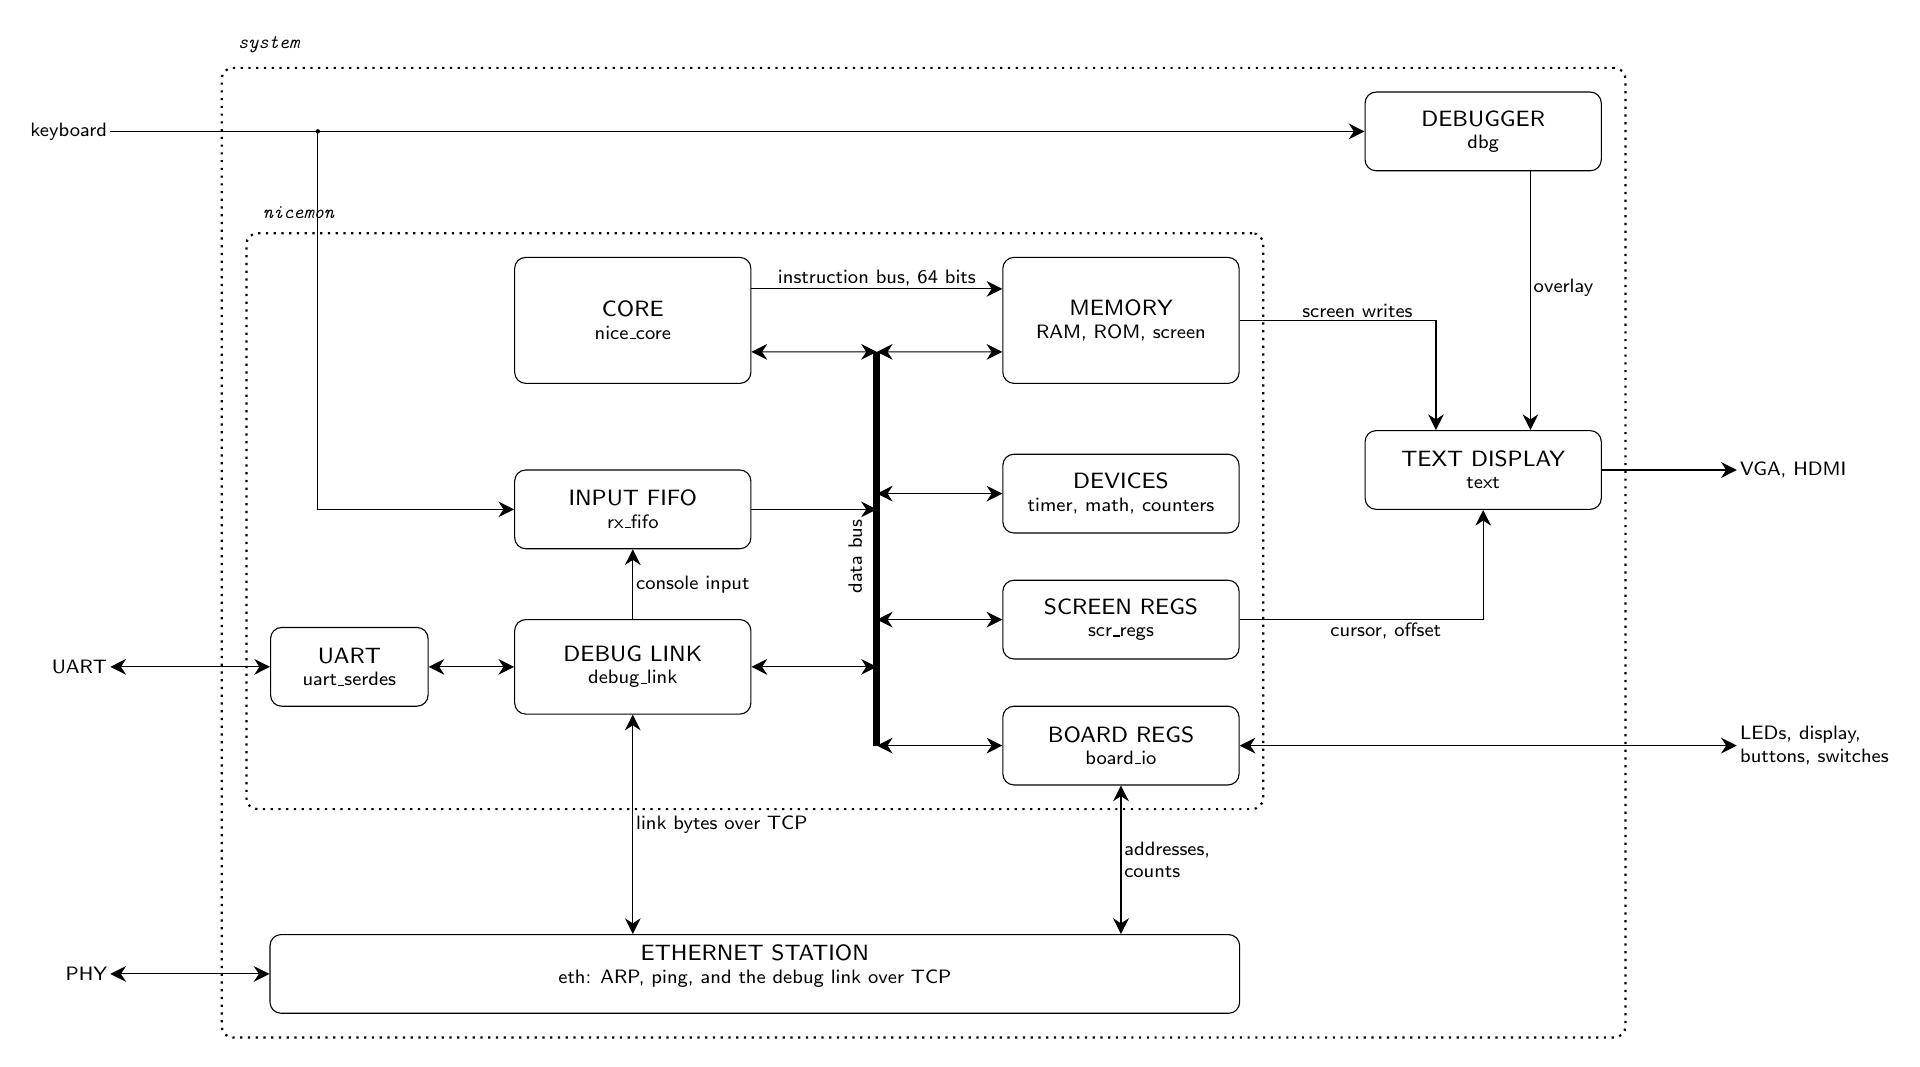
\begin{tikzpicture}[
      x = 1mm, y = 1mm,
      font = \sffamily\footnotesize,
      % A part of the system, one VHDL entity
      block/.style = {
         draw,
         rounded corners = 4pt,
         minimum width   = 30mm,
         minimum height  = 10mm,
         align           = center
      },
      sub/.style      = {font = \sffamily\scriptsize},
      wire/.style     = {draw, -{Stealth[length = 2mm, width = 2mm]}},
      both/.style     = {draw, {Stealth[length = 2mm, width = 2mm]}-{Stealth[length = 2mm, width = 2mm]}},
      wirelabel/.style = {font = \sffamily\scriptsize, align = center, inner sep = 1pt},
      % The shared data bus, drawn as a thick line
      bus/.style      = {draw, line width = 2.5pt},
      % A dotted boundary of an entity that holds others
      top/.style      = {draw, dotted, thick, rounded corners = 4pt, inner sep = 3mm},
      toplabel/.style = {anchor = south west, font = \ttfamily\scriptsize\itshape}
   ]

   %% ---------------------------------------------------------------
   %% nicemon: the masters on the left, the data bus, the slaves on the right
   %% ---------------------------------------------------------------

   \node[block, minimum height = 16mm] (core) at (0, 0)   {CORE\\[-0.5mm]
                                                           {\scriptsize nice\_core}};
   \node[block]                        (fifo) at (0, -24) {INPUT FIFO\\[-0.5mm]
                                                           {\scriptsize rx\_fifo}};
   \node[block, minimum height = 12mm] (link) at (0, -44) {DEBUG LINK\\[-0.5mm]
                                                           {\scriptsize debug\_link}};
   \node[block, minimum width = 20mm]  (uart) at (-36, -44) {UART\\[-0.5mm]
                                                           {\scriptsize uart\_serdes}};

   \node[block, minimum height = 16mm] (mem)  at (62, 0)   {MEMORY\\[-0.5mm]
                                                           {\scriptsize RAM, ROM, screen}};
   \node[block]                        (dev)  at (62, -22) {DEVICES\\[-0.5mm]
                                                           {\scriptsize timer, math, counters}};
   \node[block]                        (sreg) at (62, -38) {SCREEN REGS\\[-0.5mm]
                                                           {\scriptsize scr\_regs}};
   \node[block]                        (bio)  at (62, -54) {BOARD REGS\\[-0.5mm]
                                                           {\scriptsize board\_io}};

   % The data bus, port B of the memory and the registers
   \coordinate (busx) at (31, 0);
   \draw[bus] (busx |- 0, -4) -- (busx |- bio.west);
   \node[wirelabel, rotate = 90, anchor = south]
      at ($ (busx |- dev.west)!0.5!(busx |- sreg.west) + (-1.5, 0) $) {data bus};

   \draw[both] ([yshift = -4mm] core.east) -- (busx |- 0, -4);
   \draw[wire] (fifo.east) -- (busx |- fifo.east);
   \draw[both] (link.east) -- (busx |- link.east);
   \draw[both] (busx |- 0, -4) -- ([yshift = -4mm] mem.west);
   \draw[both] (busx |- dev.west)  -- (dev.west);
   \draw[both] (busx |- sreg.west) -- (sreg.west);
   \draw[both] (busx |- bio.west)  -- (bio.west);
   \fill (busx |- fifo.east) circle (0.8pt);
   \fill (busx |- link.east) circle (0.8pt);

   % The instruction bus, above the data bus
   \draw[wire] ([yshift = 4mm] core.east) -- ([yshift = 4mm] mem.west)
      node[wirelabel, midway, above] {instruction bus, 64 bits};

   % The link's console: the host's bytes into the FIFO, and the core's
   % bytes out through the link; the link's bytes on the UART
   \draw[wire] (link.north) -- (fifo.south)
      node[wirelabel, midway, right] {console input};
   \draw[both] (uart.east) -- (link.west);

   \node[top, fit = (core) (link) (uart) (mem) (bio)] (nicemon) {};
   \node[toplabel] at ([xshift = 1mm, yshift = 0.5mm] nicemon.north west) {nicemon};

   %% ---------------------------------------------------------------
   %% The Ethernet station and the text display
   %% ---------------------------------------------------------------

   \node[block, inner sep = 0pt,
         fit = {(uart.west |- 0, -78) (bio.east |- 0, -88)}] (eth) {ETHERNET STATION\\[-0.5mm]
         {\scriptsize eth: ARP, ping, and the debug link over TCP}};

   \draw[both] (link.south) -- (link.south |- eth.north)
      node[wirelabel, midway, right] {link bytes over TCP};
   \draw[both] (bio.south) -- (bio.south |- eth.north)
      node[wirelabel, midway, right, align = left] {addresses,\\ counts};

   \node[block] (text) at (108, -19) {TEXT DISPLAY\\[-0.5mm]
                                      {\scriptsize text}};
   \draw[wire] (mem.east) -| ([xshift = -6mm] text.north)
      node[wirelabel, pos = 0.3, above] {screen writes};
   \draw[wire] (sreg.east) -| (text.south)
      node[wirelabel, pos = 0.3, below] {cursor, offset};

   %% ---------------------------------------------------------------
   %% The on-board debugger, above the text display
   %% ---------------------------------------------------------------

   \node[block] (dbg) at (108, 24) {DEBUGGER\\[-0.5mm]
                                    {\scriptsize dbg}};
   \draw[wire] ([xshift = 6mm] dbg.south) -- ([xshift = 6mm] text.north)
      node[wirelabel, pos = 0.45, right] {overlay};

   \node[top, fit = {(nicemon) (eth) (text) (dbg)}] (system) {};
   \node[toplabel] at ([xshift = 1mm, yshift = 0.5mm] system.north west) {system};

   %% ---------------------------------------------------------------
   %% The board level, outside
   %% ---------------------------------------------------------------

   \coordinate (left)  at ([xshift = -14mm] system.west);
   \coordinate (right) at ([xshift =  14mm] system.east);

   \draw[both] (left |- uart.west) -- (uart.west);
   \node[wirelabel, anchor = east] at (left |- uart.west) {UART};
   % The keyboard's bytes go to the debugger or to the core
   \coordinate (kbdx) at (-40, 0);
   \draw[wire] (left |- dbg.west) -- (dbg.west);
   \node[wirelabel, anchor = east] at (left |- dbg.west) {keyboard};
   \draw[wire] (kbdx |- dbg.west) |- (fifo.west);
   \fill (kbdx |- dbg.west) circle (0.8pt);
   \draw[both] (left |- eth.west) -- (eth.west);
   \node[wirelabel, anchor = east] at (left |- eth.west) {PHY};

   \draw[wire] (text.east) -- (right |- text.east);
   \node[wirelabel, anchor = west] at (right |- text.east) {VGA, HDMI};
   \draw[both] (bio.east) -- (right |- bio.east);
   \node[wirelabel, anchor = west, align = left] at (right |- bio.east)
      {LEDs, display,\\ buttons, switches};

\end{tikzpicture}

\end{document}
